\documentclass[12pt,a4paper]{article}

\usepackage{mystyle}

%\loadglsentries[main]{tex/glossar}
%\makeglossaries%Glossar
%\makeindex

\begin{document}
\begin{titlepage}
\begin{center}

% Oberer Teil der Titelseite:

\includegraphics[width=0.80\textwidth]{img/oc-logo.jpg}\\[1cm]

\textsc{\LARGE Dokumentation des AI Projektes}\\[1.5cm]

\textsc{\Large Allgemeine Informatik flexibel}\\[0.5cm]
\textsc{\Large Fachhochschule Köln}\\[0.5cm]

% Title
\newcommand{\HRule}{\rule{\linewidth}{0.5mm}}
\HRule \\[0.4cm]
{ \huge \bfseries Gegenüberstellung zweier Frameworks in Bezug auf deren Tauglichkeit zur Entwicklung einer Bürgschaftsverwaltung}\\[0.4cm]
\HRule \\[1.5cm]

% Author and supervisor
\begin{minipage}{0.3\textwidth}
\begin{flushleft} \large
\emph{Author:}\\
\textsc{Mara Braun}
\end{flushleft}
\end{minipage}
\hfill
\begin{minipage}{0.5\textwidth}
\begin{flushright} \large
\emph{Unternehmen:} \\
\textsc{OPITZ CONSULTING Deutschland GmbH
Kirchstraße 6
51647 Gummersbach
www.opitz-consulting.com}
\end{flushright}
\end{minipage}

\vfill
% Unterer Teil der Seite
%{\large \today}
\end{center}
\end{titlepage}

\clearpage
%\input{./signature.tex}
\pagenumbering{roman}
\section*{Abstract}
Die OPITZ CONSULTING Deutschland GmbH ist seit einigen Jahren mit der Wartung einer Webanwendung zur Verwaltung von Bürgschaften betraut. Da diese Anwendung jedoch schon vor einigen Jahren entwickelt wurde entspricht ihre Performanz nicht mehr den Anforderungen der heutigen Zeit. Daher soll die Anwendung neu entwickelt werden. Hierfür kommen zwei große Frameworks in Frage. Das erste Framework ist das Application Development Framework von Oracle, in dessen veralteter Version  die zugrunde liegende Anwendung ursprünglich erstellt wurde. Das zweite Framework ist das zur Zeit verbreitete Framework Grails.

Im Folgenden Dokument sollen nun die beiden Frameworks miteinander verglichen werden. Dieser Vergleich soll die Vor und Nachteile der beiden Frameworks gegenüberstellen, um zu evaluieren, welches sich besser zur Neuentwicklung der Bürgschaftsverwaltung eignet.
\tableofcontents
\listoffigures
%\listoftables
\clearpage
\pagenumbering{arabic}
\section{Einleitung}
Im Zeitalter des Internets sind Web Anwendungen und mit ihnen Web Application Frameworks immer beliebter geworden, weshalb es zur heutigen Zeit eine Vielzahl von Web Application Frameworks gibt. Dies erschwert die Auswahl eines geeigneten Frameworks für das eigene Projekt, was auch allgemein ein relavantes Thema in Softwarehäusern, wie z.B. der OPITZ CONSULTING Deutschland GmbH ist. Die OPITZ CONSULTING Deutschland GmbH ist seit einigen Jahren mit der Wartung der unterschiedlichsten Anwendungen betraut und erhält ebenfalls regelmäßig Aufträge zur Entwicklung neuer Software. Zu den zu wartenden Anwendungen gehört unter anderem die Web Anwendung "`AvaleNet"' eines Bankhauses, die in einer veralteten Version des Frameworks Application Development Framework (ADF) entwickelt wurde und nun neu entwickelt werden soll, da die Performanz der Anwendungen nicht mehr den Ansprüchen der heutigen Zeit genügt. Hierzu muss nun eine Entscheidung getroffen werden, welches Framework zur Migration der Anwendung verwendet werden soll. Die Entscheidungsfindung, welches der beiden zur Auswahl gestellten Frameworks verwendet werden soll, ist Bestandteil des folgenden Dokumentes. Hierfür werden zunächst die fachlichen Details der beiden Frameworks erläutert, um im darauf folgenden Kapitel die Vor- und Nachteile der beiden Frameworks besser nachvollziehen zu können. Diese Vor- und Nachteile, die mit Hilfe einer zur Vergleichbarkeit entwickelten Metrik ermittelt wurden, werden dann in Bezug zu der zu entwickelnden Anwendung "`AvaleNet"' gesetzt und gegenübergestellt. Zuletzt wird eine Gewichting der einzelnen Kriterien vorgenommen, anhand derer letztendlich entschieden wird, welches Framework sich am besten zur Migration der Anwendung eignet.
\section{Theoretische Grundlagen}
Dieses Kapitel soll für ein grundlegendes Verständnis der Architektur von ADF und Grails und dem Umfang dieser Frameworks sorgen, um im nachfolgenden Vergleich der beiden Frameworks die Vor und Nachteile nachvollziehen zu können.
\subsection{Entstehung}
Mit der Einführung von SOA (Service Oriented Architecture) in der Softwareentwicklung hat die Entwicklung von traditionellen Webanwendungen, in denen die Anwendung eine vollständige Lösung ist ein Ende gefunden. Moderne Anwendungen sind heute nicht mehr eine vollständige Lösung, sondern sie sind komponentenbasierte Benutzerschnittstellen, die lokale und remote Services für ihre Business Logik verwenden. (Oracle Fusion Developer Guide Introduction Seite xxi)
\subsection{MVC Architektur allgemein}
Dieses Kapitel soll dazu dienen, ein Verständnis für die den beiden Frameworks zu Grunde liegenden Architektur zu schaffen.\\


Die Model View Controller (MVC) Architektur wurde in den 1970er Jahren von Trygve Reenskaug für die Plattform Smalltalk entwickelt und spielt bis heute eine bedeutende Rolle in den meisten UI-Frameworks und dem UI-Design.
Wie der Name schon vermuten lässt, besteht die MVC Architektur aus drei Rollen, dem Model, dem View und dem Controller.
\begin{itemize}
\item Das Model ist ein nicht sichtbares Objekt, dass einige Informationen der Domäne, wie z.B. alle Daten und Verhalten enthält. Diese Daten und Informationen müssen nicht denen die in der UI verwendet werden entsprechen.

\item Die View dient dazu Informationen aus dem Model anzeigen zu können. Dies kann z.B. in Form einer HTML-Seite geschehen, in der die gewünschten Informationen des Models dann angezeigt werde.

\item Die letzte Rolle ist die des Controllers. Der Controller dient dazu Benutzereingaben anzunehmen, das Model zu manipulieren und das View Objekt zu aktualisieren.
\end{itemize}
Die wichtigste Trennung ist die Trennung von Model und View. Der Grundgedanke hierbei ist es, dass ein Entwickler wenn er eine View (Ansicht) entwickelt über andere Dinge nachdenkt, als wenn er das Model entwickelt. Beispielsweise denkt er bei der Entwicklung der View mehr über die Mechanisemen der UI nach und bei der Entwicklung des Models mehr über die Geschäftsstrategie nach. Zudem möchte ein User eventuell ein und die selbe Information aus dem Model in einer Anwendung auf unterschiedliche Weise dargestellt haben, was sich durch die Trennung von View und Model vereinfacht, da für jede Ansicht das selbe Model verwendet werden kann und sich nur die View ändert. Ein letzter Aspekt, der für die Trennung von Model und View spricht, ist das nicht sichtbare Objekte meist besser zu testen sind als sichtbare und so durch die MVC-Architektur die Modellogik getrennt von der Benutzeroberfläche (GUI) getestet werden kann.\\
Die Trennung von View und Controller dagegen ist weniger relevant, weshalb in einigen Frameworks heute eine Kombination von View und Controller verwendet wird. Selbst in den meisten Versionen von Smalltalk, für die die MVC-Architektur ursprünglich entwickelt wurde, wurde meiste eine Kombination von View und Controller verwandt. Die Trennung von View und Controller ist vorallem dann sinnvoll, wenn er sich um Rich-Client-Systeme handelt oder der Controller von Web-Frontends separiert wird.\\
\begin{figure}
\centering
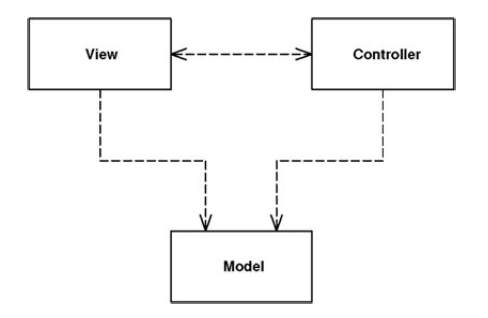
\includegraphics[width=0.80\textwidth]{img/MVC-Allgemein(Fowler).png}
\caption {MVC-Architektur}
\end{figure}
Wie auch in der Abbildung zu sehen, ist die Richtung der Abhängigkeiten für die MVC-Architektur entscheidend. Die Abbildung zeigt, dass sowohl View als auch Controller vom Model abhängig sind, jedoch keine Abhängigkeit des Models von View oder Controller besteht. Diese Unabhängigkeit des Models bedeutet, dass das Model auch bei Änderungen an View und Controller unverändert bleibt und damit Änderungen am View deutlich erleichtert.
(Patterns of Enterprise Application Architecture - Martin Fowler)
\subsection{ADF}
Dieses Kapitel soll einen Einblick in die Möglichkeiten des Frameworks ADF bieten und dessen Aufbau und Bedienbarkeit erläutern.

\subsubsection{Grundlegendes}

Eine Lösung zur Entwicklung von modernen Anwendungen als komponentenbasierte Benutzerschnittstelle bietet ORACLE mit dem Application Development Framework (ADF). ADF ist ein Java EE (Java Enterprise Edition) Framework, das Anwendungsentwicklung mit Java, Java EE und SOA vereinfachen soll um ein breites Publikum von Geschäftsbereich und Technologie Experten anzusprechen, die zusammen arbeiten müssen, um langlebige Enterprise Softwarelösungen entwickeln zu können.(Oracle Fusion Developer Guide Introduction Seite xxiii)
\subsubsection{Architektur}
\begin{figure}
\centering
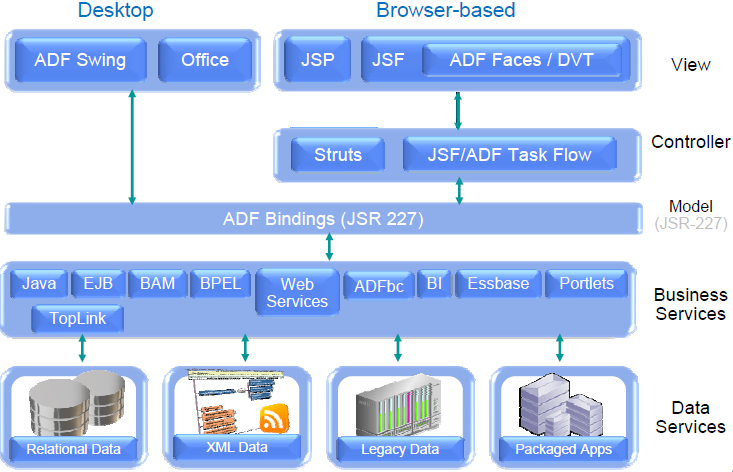
\includegraphics[width=0.80\textwidth]{img/MVC-ADF.png}
\caption {MVC-Architektur von ADF}
\end{figure}
\subsection{Grails}
Dieses Kapitel soll einen Einblick in das Framework Grails ermöglichen.

\section{Gegenüberstellung der Frameworks}
\subsection{Anforderungen an Web Application Frameworks}
Dieses Kapitel soll die wesentlichen Anforderungen an Web Application Frameworks ausführen und eine Begründung enthalten, weshalb diese Anforderungen relavant sind. Es wird benötigt, um in den folgenden Kapiteln die Vor- und Nachteile der beiden Frameworks vergleichbar darstellen zu können.
\subsubsection*{Lizenz und Lizenzkosten}
Da es sowohl Open Source als auch lizenzierte Frameworks zur Entwicklung von Webanwendungen gibt, können sich die eventuell vorhandenen Lizenzkosten auf die Gesamtkosten des Projektes auswirken. Zudem müssen anfallende Lizenzkosten zum Betreiben der entwickelten Software bei der Auswahl eines Frameworks mit betrachtet werden.
Ein weiterer zu beachtender Punkt bezüglich der Lizenzen ist die GNU General Public License (GNU GPL), denn sobald Teile des Quellcodes einer Software die unter diese Lizenz fällt in der eigenen Anwendung verwendet werden kann die Notwendigkeit bestehen, dass die eigene Anwendung ebenfalls unter diese Lizenz fallen muss. Daher ist insbesondere bei der Verwendung von GNU GPL Erweiterungen zu prüfen ob die Anwendung bei Verwendung ebenfalls unter die GNU GPL fällt.
\subsubsection*{Entwicklungsgeschwindigkeit}
Die mögliche Geschwindigkeit mit der mit einem Framework entwickelt werden kann ist sehr entscheidend bei der Wahl des Frameworks, da die Entwicklungszeit und damit auch die Kosten für den Kunden möglichst gering gehalten werden sollen. Aus diesem Grund sollte auf diesen Aspekt geachtet werden. In die tatsächliche Entwicklungsdauer fließt jedoch auch noch die Lernkurve mit ein.
\subsubsection*{Lernkurve}
Da Web Application Frameworks nicht alle gleich aufgebaut oder ähnlich umfangreich sind, kann auch die Einarbeitungszeit für das entsprechende Framework unterschiedlich lang ausfallen. Da dies die Entwicklungszeit für die entsprechende Software verlängern oder verkürzen kann, gilt es die Lernkurve bei Auswahl des Frameworks zu beachten.
\subsubsection*{Community}
Für die Entwicklung mit einem entsprechenden Framework kann die vorhandene Community ein essentieller Bestandteil sein, denn immer wieder können bei der Entwicklung Fehler oder Probleme auftreten, deren Lösung viel Zeit in Anspruch nehmen kann. In einer großen Community kann das Problem aber bereits von einem anderen Entwickler gelöst und festgehalten worden sein oder aber es wird auf Anfrage von jemandem gelöst, was einiges an Zeit einsparen kann.
\subsubsection*{Testbarkeit}
Die Testbarkeit von Software ist allgemein sehr wichtig, da Software zum einen komplex ist und sich zum anderen häufig ändern kann. Auf Grund dieser beiden Aspekte, ist es möglich, dass durch Änderungen Fehler entstehen können die in der komplexen Software vielleicht zunächst nicht auffallen. Eine gute Testabdeckung kann verhindern, dass solche Fehler übersehen werden.
\subsubsection*{Umfang und Qualität der Dokumentation}
Eine umfangreiche und verständliche Dokumentation ist sehr wichtig um mit dem Framework arbeiten zu können. Eine schlechte Dokumentation führt schnell zu Verwirrung und Frustration und verlangsamt damit auch die Entwicklungsgeschwindigkeit. Eine umfangreiche und mit Beispielen versehene Dokumentation ist daher wichtig für die Auswahl des Frameworks.
\subsubsection*{Modularität}
Da es sehr viele verschiedene Verwendungsmöglichkeiten für Web Anwendungen mit sehr unterschiedlichen Funktionsanforderungen gibt, ist es häufig sinnvoll nicht alle möglichen Funktionalitäten im Framework zu integrieren, sondern diese durch Erweiterungen (im nächsten Punkte näher erläutert) verfügbar zu machen. Ein leichtgewichtigeres Framework ist für kleine Webanwendungen daher besser geeignet, da weniger nicht benötigte Funktionen enthalten sind und die Komplexität des Frameworks nicht unnötig vergrößern.
\subsubsection*{Erweiterbarkeit}
Bei der Entwicklung einer Web Anwendung ist es gut möglich, dass Funktionen verwendet werden sollen, die für sehr viele Web Anwendungen die selben sind (z.B. die Authentifizierung). Daher ist die Erweiterbarkeit des Frameworks und die Möglichkeit der Verwendung von Plugins für Web Application Frameworks ein wesentlicher Aspekt.
\subsubsection*{Versionierbarkeit}
Da Software und damit auch Webanwendungen häufig im Team entwickelt werden, muss eine Möglichkeit zur Versionierung der zu entwickelnden Anwendung gegeben sein. Hierbei ist es wünschenswert, dass beim Zusammenführen der verschiedenen Entwicklungsstände möglichst wenig Konflikte auftreten. Weiterhin sollte gute Versionierung Änderungen im Nachhinein nachvollziehbar machen.
\subsubsection*{Langlebigkeit}
Die Langlebigkeit eines Frameworks ist insbesondere im Bezug auf den zugehörigen Support und Sicherheitsupdates relevant, da diese mit dem Aussterben des Frameworks ebenfalls wegfallen. Es ist also für eine Anwendung die für eine lange Dauer zum Einsatz kommen soll zu beachten, dass auch das Framework für diese Dauer warscheinlich weiterhin unterstützt wird.
\subsubsection*{Performanz}
Die Performanz von Web Application Frameworks und den daraus resultierenden Anwendungen ist ebenfalls ein wesentlicher Punkt bei der Auswahl eines Frameworks, jedoch wird dieser hier nicht genauer betrachtet, da es schwer ist sinnvoll vergleichbare Werte für die Performanz zweier Frameworks zu finden.
\subsection{Vor- und Nachteile von ADF}
Dieses Kapitel soll die Vor- und Nachteile von ADF anhand des zuvor aufgestellten Anforderungskatalogs erläutern und hervorheben, inwiefern sich ADF von anderen Web Application Frameworks abhebt.\\\\
Da ADF eine proprietäre kommerzielle Software ist fallen bei Einsatz der, mit diesem Framework entwickelten, Software Lizenzkosten an. Jedoch hat die Verwendung eines proprietären Frameworks den Vorteil, das der Quellcode in keinem Fall offen gelegt werden muss, wie es bei der GNU GPL\footnote{https://www.gnu.org/copyleft/gpl.html} der Fall ist, was für einige Kunden essentiell ist. Der Aufbau des Frameworks ADF lässt jedoch nicht als modular bezeichnen, da ADF ein kaum erweiterbares Framework ist und entsprechend den gesamten Umfang der möglichen Funktionen schon zu Beginn enthält. Dieser große Umfang des Frameworks wirkt sich wiederum auf die Lernkurve des Frameworks aus und bewirkt, dass das Framework insbesondere für Entwickler mit wenig Erfahrung im Java Enterprise Umfeld schwerer zu erlernen ist. Einen Überblick über das Framework ADF zu bekommen kann daher einiges an Zeit erfordern und wirkt sich damit negativ auf die Entwicklungsdauer aus. Einem Entwickler, der bereits Erfahrung mit ADF gesammelt hat und mit ADF vertraut ist, ist das sogenannte "`Rapid Application Development"' möglich, das ADF durch seinen baukastenartigen Aufbau und die vielen Wizards ermöglicht. Dieses schnelle Entwicklungstempo wird zudem durch die umfangreiche Dokumentation und den Support von Oracle selbst durch zahlreiche Tutorials für die unterschiedlichsten Problemszenarien unterstützt. Die zu ADF gehörige Community ist weltweit deutlich kleiner als die zum Framework Grails gehörige. Dies lässt sich anhand der folgenden Abbildung erkennen. 
\begin{figure}[h]
\centering
\includegraphics[width=\textwidth]{img/interesse_zeitl.png}
\caption{Zeitverlauf des Interesses an ADF und Grails weltweit (Quelle: \GoogleTrends) }
\end{figure}
Die Grafik zeigt den zeitlichen Verlauf des Interesses an den beiden Frameworks ADF (in rot) und Grails (in blau) weltweit anhand der Häufigkeit\footnote{für genauere Erläuterung zur Wertefindung im Diagramm: http://goo.gl/Ma9kWJ} von Suchanfragen über Google. Das Suchinteresse wird hierbei relativ zum Höchstwert dargestellt. Diese Grafik lässt den Schluss zu, dass ADF zwar eine kleinere Community hat aber sich durchaus als langlebig erwiesen hat, das das Interesse an ADF mehr oder weniger konstant bleibt. Die Langlebigkeit des Frameworks, die auch in Zukunft zu erwarten ist bietet den Vorteil, dass auch der Support weiterhin besteht und damit auch spätere Wartungsaufgaben erfüllbar sind. Auch die im Anforderungskatalog aufgeführten Punkte Versionierbarkeit und Testbarkeit erfüllt ADF, da es sich zum einen mit den bekannten Versionierungstools GIT und SVN versionieren lässt und damit auch die Arbeit in größeren Teams zulässt, zum anderen aber auch beispielsweise Unit Tests möglich sind um z.B. selbst erstellte Java Klassen und Methoden testen zu können. Bei der Versionierbarkeit gilt es jedoch zu beachten, dass nicht jeder Schritt für andere Entwickler Nachvollziehbar bleibt, da ADF viele Wizards zur Erstellung von Funktionen, Klassen und Dateien bietet. Diese Wizards sind aus der Sicht von GIT und SVN die rein textbasiert arbeiten nicht nachvollziehbar.

\subsection{Vor- und Nachteile von Grails}
Dieses Kapitel soll die Vor- und Nachteile von Grails anhand des zuvor aufgestellten Anforderungskatalogs erläutern und herhorheben, inwiefern sich Grails von anderen Web Application Frameworks abhebt.\\\\
Grails ist ein modulares Open Source Framework, dass unter die Apache License in der Version 2.0\footnote{http://www.apache.org/licenses/LICENSE-2.0.html} fällt. Diese Lizenz hat zunächst keine Auswirkungen auf die zu entwickelnde Anwendung, da im allgemeinen diese Lizenz nur eine Auswirkung hätte, wenn das Framework Teile des eigenen Source Codes in das Programm kopieren würde. Dies kann aber bei Grails höchstens bei Plugins (den zahlreichen Erweiterungsmöglichkeiten von Grails) vorkommen, die wiederum alle ihre eigenen Lizenzen haben. Dies hat wiederum den Nachteil, dass man für jede der vielen möglichen Erweiterungen des Frameworks, die man verwenden möchte zunächst überprüfen muss ob die Lizenz Auswirkungen auf die zu entwickelnde Software hat. Diese Überprüfungen können wenn sie notwendig sind, negative Auswirkungen auf die Entwicklungsgeschwindigkeit haben. Ansonsten sind Entwicklungsgeschwindigkeit und Lernkurve für Entwickler mit Java Vorkenntnissen sehr gut, da diese Grails schnell lernen können und entsprechend schnell entwickeln können. Grails bietet allerdings weniger Wizards und ist nicht wie ADF nach dem Baukasten Prinzip für "`Rapid Application Development"' ausgelegt. Es muss also der meiste Code selbst geschrieben werden. Durch sehr viel selbst geschriebenen Code wird sowohl eine umfangreiche Testabdeckung, als auch eine gute Dokumentation und Commmunity benötigt. Diese Punkte sind gegeben, da Grails die Java basierte Programmmiersprache Groovy verwendet und damit zum einen die gleichen Testmöglichkeiten bestehen, zum anderen aber auch die Javadocs als Dokumentation gültig sind, welche sehr umfangreich sind. Zusätzlich zu der Java Dokumentation hat Grails aber auch eine eigene umfangreiche Dokumentation und eine große Community, die in entsprechenden Foren Fragen beantwortet und Beispiele für verschiedene Problemstellungen zur Verfügung stellt. Wie auch für ADF lässt sich die Größe der Community etwa am Zeitverlauf des Interesses an den beiden Frameworks und an den Einträgen in dem wohl meist genutzten Portal "`Stackoverflow"'\footnote{http://stackoverflow.com/questions/tagged/grails} ablesen. Was die Langlebigkeit von Grails betrifft so ist das Interesse an Grails weniger konstant, jedoch ist es hoch genug um davon ausgehen zu können, dass Grails noch einige Zeit bestehen wird. Ein Weiterer für Webapplication Frameworks relevanter Punkt ist die Versionierbarkeit. Das Versionieren der zu entwickelnden Software via z.B. SVN oder GIT ist problemlos möglich. Hierbei hat Grails jedoch den Vorteil, dass durch den vielen eigenen Code und weniger Wizards die ausgeführten Schritte später leichter nachzuvollziehen sind, was für Entwicklung in großen Teams ein großer Vorteil ist.
\section{Fazit}
Dieses Kapitel fasst noch einmal zusammen, weshalb das Framework gewählt wurde und welches nach der Gegenüberstellung besser zur Entwicklung geeignet ist.
\clearpage
\addcontentsline{toc}{section}{Literaturverzeichnis}
\section*{Literaturverzeichnis}
%\printglossary[title=Glossar]%Glossar ausgeben
\clearpage
%\input{tex/anhang}
\end{document}

%%% Local Variables:
%%% mode: latex
%%% TeX-master: t
%%% End:
